\section{Technologies d'indoor positioning}

Dans cette partie il s'agira de faire une liste des technologies d'indoor positionning. Ces technologies sont divisées en deux grandes catégories, à savoir celles basées sur les ondes radiofréquences et celles basées sur l'imagerie.
\subsection{Technologies basées sur les ondes radiofréquences}


\subsubsection{WiFi}

Le Wi-Fi est un ensemble de protocoles de communication sans fil regroupés sous la norme IEEE 802.11.
Dans le cadre l'indoor positioning il est utilisé dans une configuration composée de :
\begin{itemize} 
\item Une zone de détection définie
\item Un tag, à savoir l'objet à positionner
\item Des anchors ou balises Wi-Fi 
\end{itemize}
\begin{figure}[H]
    \centering
    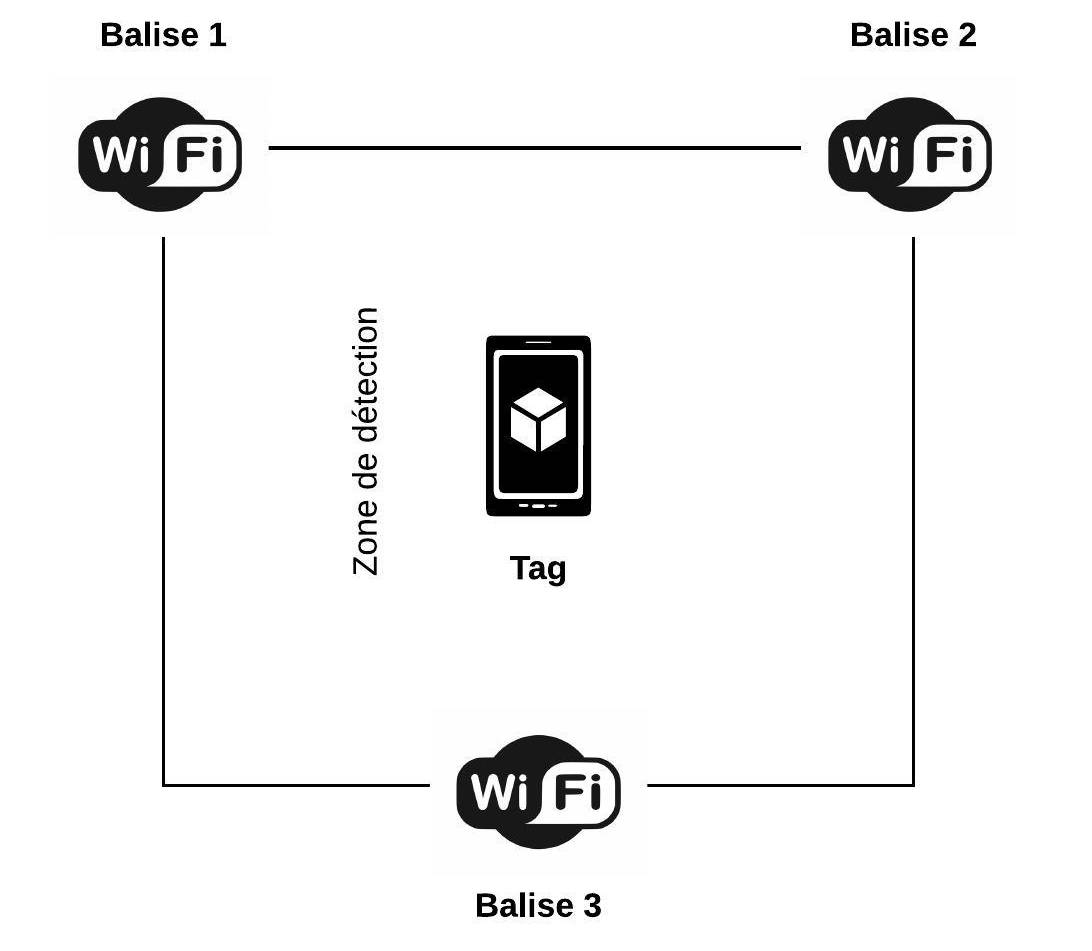
\includegraphics[width=0.7\textwidth]{\pathTech/tech0.jpeg}
    \caption{Systeme d'indoor positionning utilisant le Wi-Fi.}
\end{figure}
Ici, le tag et la balise vont communiquer afin de permettre la localisation. 
Le Wi-Fi peut être utilisé de deux manières différentes dans le cadre l'indoor positioning.
\begin{itemize} 


    \item Mode récepteur : Toutes les balises environnantes émettent vers le tag. Les ressources de calcul
    requises au niveau du tag sont accrues, mais cela permet une mise à jour quasi immédiate de la position, car
    aucune ressource externe n’est nécessaire.
    \item Mode émetteur : seul le tag est chargé d’émettre à destination des anchors environnants. Les
    ressources de calcul requises au niveau du tag s'en trouvent réduites, mais la mise à jour de la position dépendra ici de plusieurs éléments et non d'un seul comme précédemment ce qui nécessite un synchronisation des tous les composants.
\end{itemize}
Le principal avantage du Wi-Fi est qu'il est relativement peu cher et présent partout, que ce soit dans les foyers, les écoles ou les centres commerciaux par exemple.
Il a aussi une portée conséquente allant de 150m jusqu'à 250m.
\medskip
\\
Cependant cette technologie admet une faible précision dans les zones qui ne sont pas neutres, sans interférences. On parle d'une précision allant de 5 à 10 mètres pour ces zones.
\medskip
\\
D'un point de vue économique le Wi-Fi est peu cher, il est possible de mettre en place des systèmes décrits ci-dessus avec des Raspberry Pi dont le prix est d'environ 37 euros l'unité.
\subsubsection{BLE}
Le BLE ou Bluetooth Low Energy est une technique de transmission sans fil basse consommation regroupée sous le standard Bluetooth.
Il est utilisé dans une configuration similaire à celle du Wi-Fi.
Le tag sera ici majoritairement un smartphone ou une tablette, car ces derniers embarquent déjà les capteurs nécessaires.
\\
Le principal avantage du BLE est bien évidemment son prix et sa présence auprès des smartdevices. Sa faible consommation énergétique est aussi un avantage non négligeable dans le domaine de l'IoT.
\medskip
\\
Comme le Wi-Fi, c'est la précision qui fait défaut au BLE, on parle ici d'une précision allant de 2m à 10m. À titre informatif la portée de cette technique va de 10m à 100m.
\medskip
\\
D'un point de vue économique le BLE est encore une fois peu cher. L'achat de dongles BLE coûte aux alentours d'une dizaine d'euros pièces.
\subsubsection{UWB}
L'UWB ou Ultra Wideband, est un nouveau type de modulation radio sans fil. Ce dernier est caractérisé par une grande largeur de bande par rapport à la fréquence centrale des ondes émises. Sa large bande passante permet une résolution temporelle précise et sa faible fréquence offre une meilleure pénétration des ondes à travers les matériaux.
\begin{figure}[H]
    \centering
    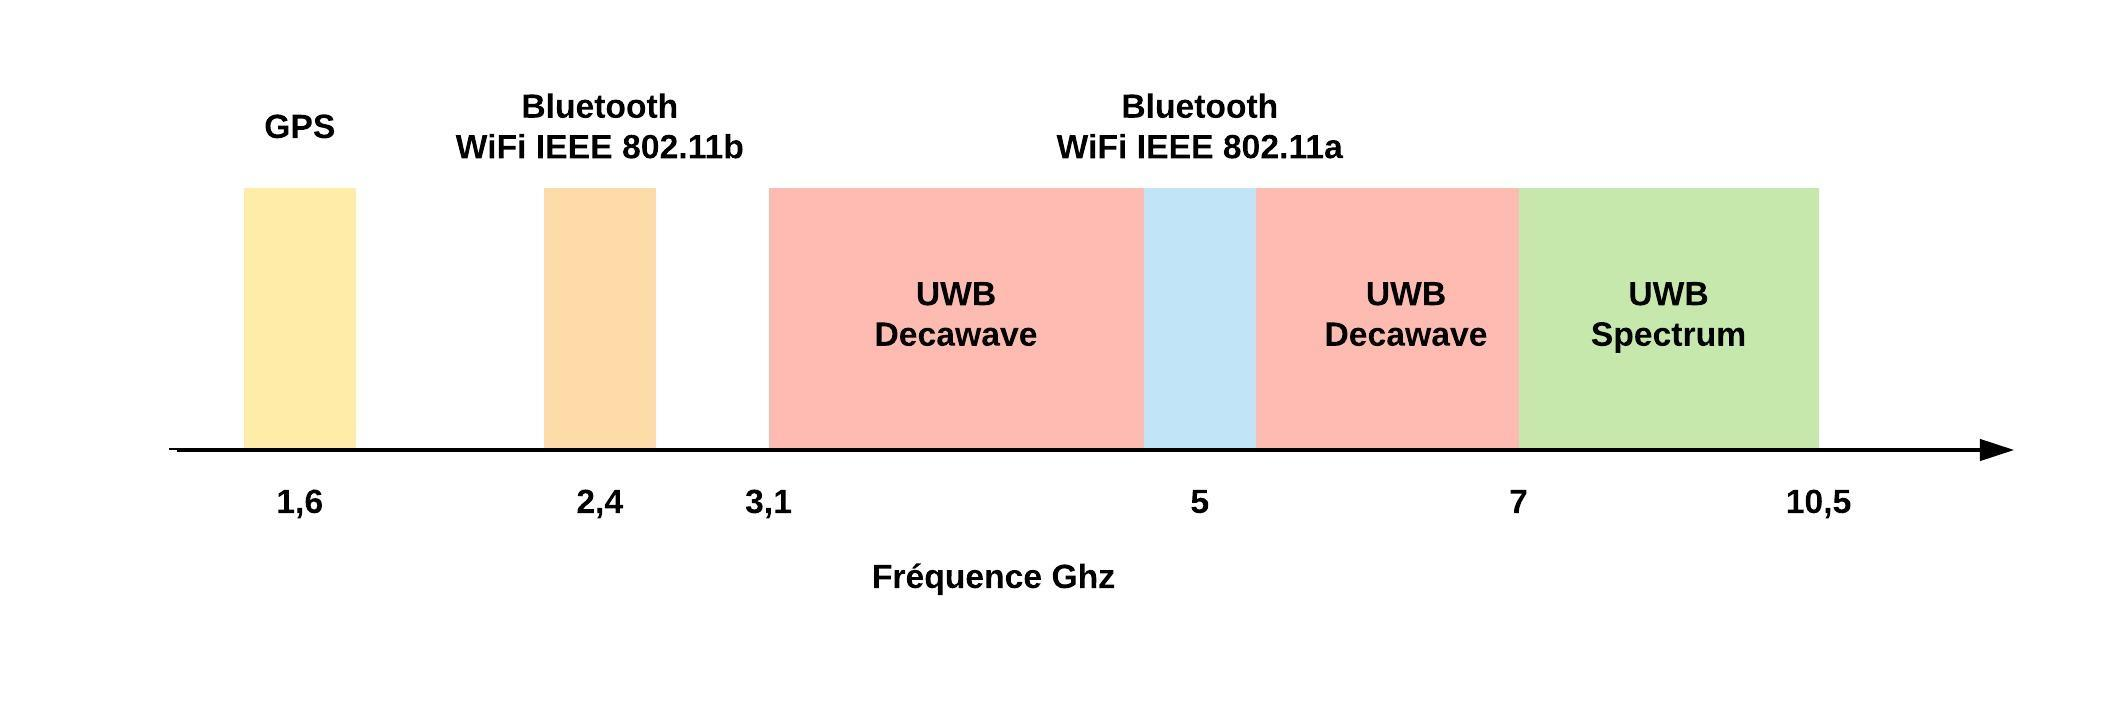
\includegraphics[width=1\textwidth]{\pathTech/UWB.jpeg}
    \caption{Comparaison fréquentielle entre le GPS le Bluetooth, les Wi-Fi, et les UWB.}
\end{figure}

Les avantages de l'UWB sont sa haute précision, de l'ordre de 15 cm ainsi que sa forte adaptabilité à l'environnement. 
Cependant cette technologie n'est encore qu'en phase expérimentale pour une utilisation commerciale. De ce fait il n'existe que très peu de documentation rendant compliquée une exploration précise.
\\
D'un point de vue économique un module UWB est relativement abordable. Son prix avoisine les 25 euros pièce pour un module Decawave Sensor UWB.
L'utilisation est similaire au BLE ou au WiFi. Il faut bien évidemment ajouter à ceci un microcontrôleur qui effectuera les calculs nécessaires.


\subsubsection{Ultrasons}

L'ultrason est une onde mécanique élastique dont la fréquence est située entre 16 kHz et 10 MHz. Son utilisation dans des systèmes de localisation est majoritairement couplée avec l'utilisation de son dont la fréquence est plus élevée.
Le système cricket illustre parfaitement cette combinaison.
\\
Dans ce système, deux émetteurs, un sonore et un ultrasonore, émettent en même temps une salve d'ondes.
Le tag à localiser reçoit en premier l'onde ultrasonore, car plus rapide et déclenche un compteur qui s'arrêtera lors de la réception de l'onde sonore plus lente.
Connaissant la vitesse de propagation des deux et le temps écoulé entre les deux réceptions, on déduira sans grande difficulté la distance qui sépare l'émetteur du tag.
On déduira par la suite à position exacte du tag avec une méthode de triangulation.
\begin{figure}[H]
    \centering
    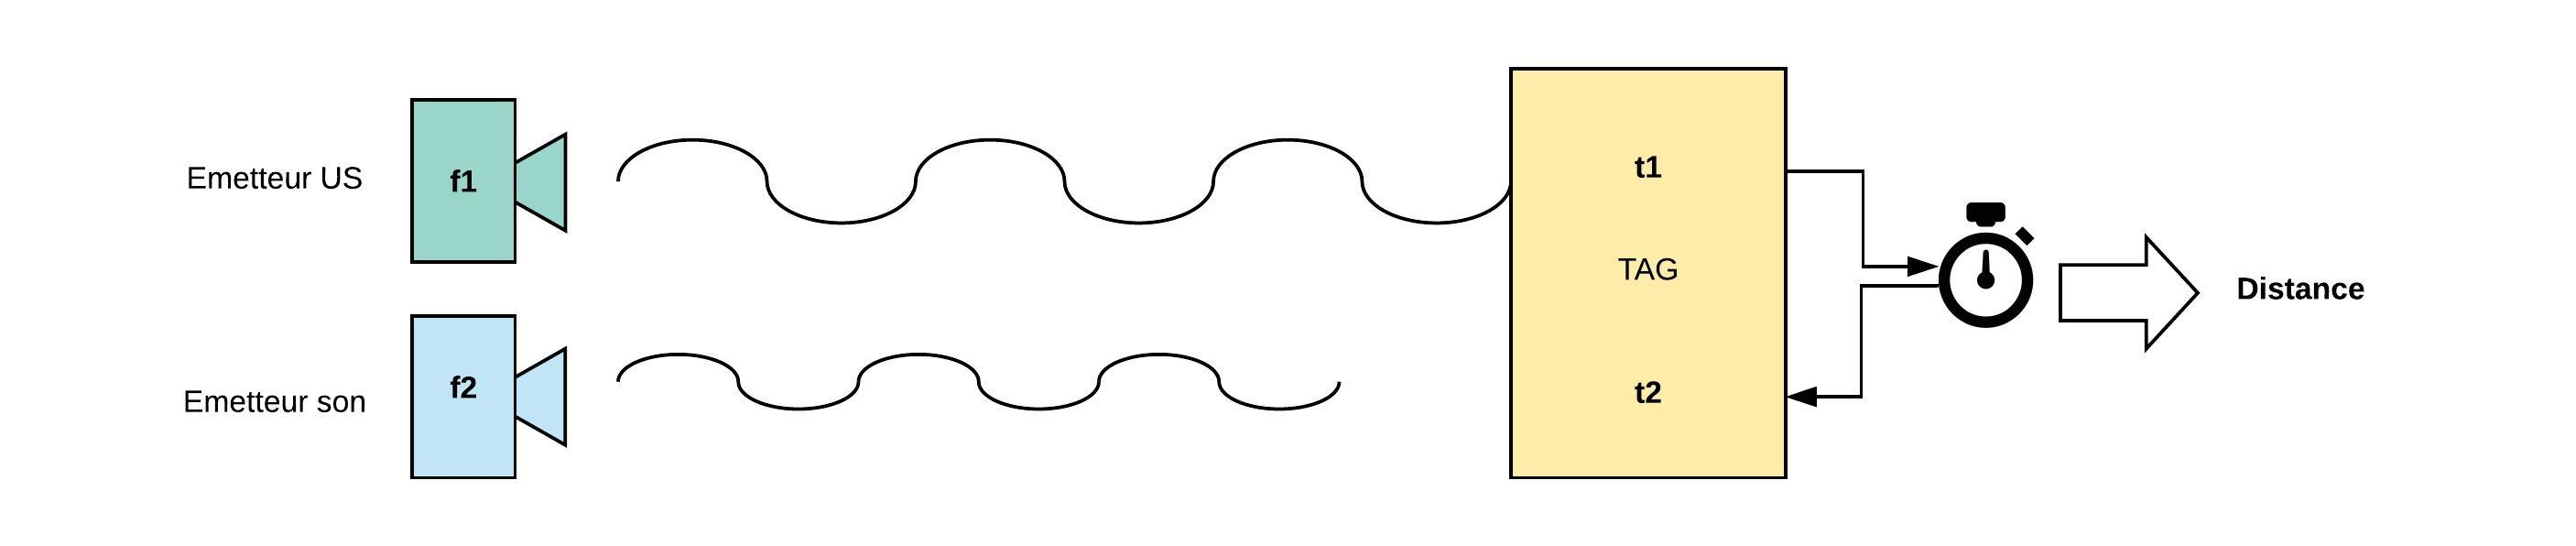
\includegraphics[width=1.1\textwidth]{\pathTech/US.jpeg}
    \caption{Le système "Cricket" basé sur les ondes ultrasonores.}
\end{figure}
Le principal avantage de cette technique est sa précision, en effet avec l'utilisation d'ultrason on atteint une position à la dizaine de centimètres près.
\medskip
\\
Cependant, cette technique n'est précise que sur les courtes distances et dans des zones neutres de toutes perturbations, ces dernières pouvant fausser les calculs.
\medskip
\\
Pour ce qui est du prix un émetteur à ultrasons coûte entre 5 et 10 euros. Il faudra ajouter à ce prix celui d'une carte de type Raspberry ou Arduino pour créer un émetteur ultrasonore fonctionnel. 
\subsubsection{Champ magnétique}
L'étude du champ magnétique a toujours été source de recherches tant son utilisation est diverse.
Son utilisation dans la géolocalisation en intérieur nécessite une cartographie du lieu, c'est à dire un relevé de valeurs en différents points de l'espace qui seront ensuite sauvegardés dans une base de données. 
On parle ici de fingerprint.
Il s'agira ici d'effectuer des relevés de la puissance du champ magnétique pour pouvoir se localiser.
\medskip
\\
L'avantage principal de cette technique est qu’elle ne nécessite pas d'infrastructure. Ici il s'agira seulement de développer le système d'acquisition du champ magnétique.
\medskip
\\
Cependant la précision de cette technique lui fait défaut, on parle ici d'une précision allant de 30 cm jusqu'a quelques mètres. La présence d'objets métalliques peut aussi grandement fausser le résultat.


\subsection{Technologies basées sur l'imagerie}
\subsubsection{Spectre visible}
Toutes les techniques de localisation basées sur le spectre visible sont des techniques de détection de contours et d'environnement. 
Ici une caméra se chargera de l'acquisition de l'image et un algorithme permettra le traitement de l'image.
Avec la démocratisation de la machine learning, il est tout à fait concevable d'utiliser un tel algorithme afin d'accroitre les performances de la localisation.
\begin{figure}[H]
    \centering
    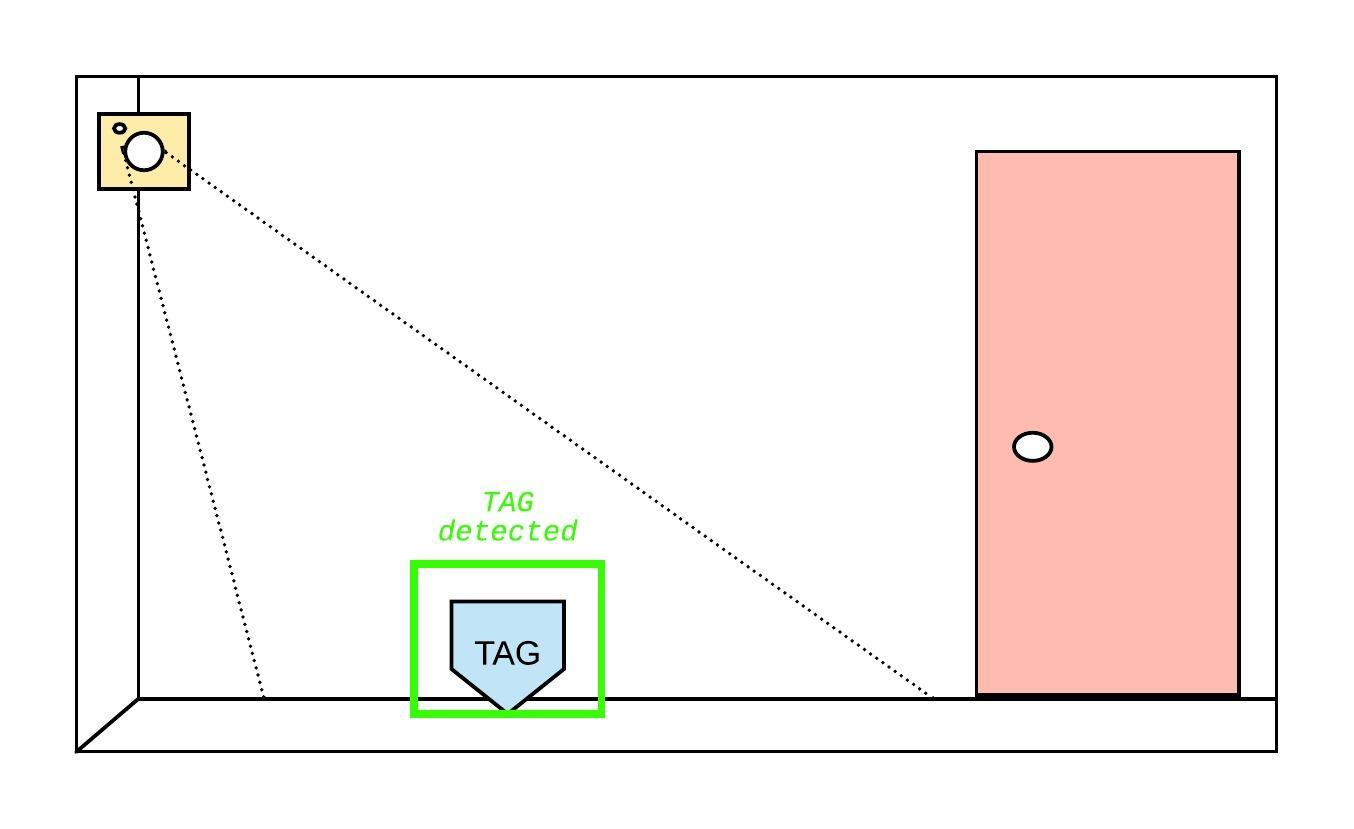
\includegraphics[width=0.8\textwidth]{\pathTech/visible.jpeg}
    \caption{Principe de mise en place d'un système de localisation grâce au spectre visible.}
\end{figure}
Les avantages liés à cette technique sont la rapidité d'implémentation de la méthode ainsi que sa précision, on parle ici d'une précision de l'ordre de 5cm.
\\
Cependant, une telle méthode nécessite que l'objet à localiser soit en vue de la caméra, hors du champ de cette dernière, le calcul localisation est impossible. De même, les interférences avec des objets venant obstruer la vue de l'objet posent un souci d'identification.
\medskip
\\
Sur le plan financier l'utilisation de cette technique nécessite l'achat d'une caméra, ici une webcam fera amplement le travail. On peut en trouver aux alentours de 20-30 euros.
\subsubsection{Spectre IR}
Le rayonnement infrarouge est un rayonnement électromagnétique dont les longueurs d'onde sont comprises entre 700 nm et 1 mm. Dans le cadre de la localisation, on distingue deux grandes techniques basées sur l'IR.
\begin{itemize} 
\item On place une série d'émetteurs LED, infrarouges autour de la zone de détection souhaitée et on place sur le tag un détecteur d'infrarouges. En fonction des angles des réceptions des différents LED, on pourra en déduire sa position dans l'espace.
\item On place sur un robot des émetteurs et des récepteurs infrarouges dans différentes directions. On effectue un balayage de la zone de détection avec le robot et ce dernier reconstituera cet environnement en une cartographie 2D ou 3D grâce aux ondes reçues. Un outil comme le scanner LIDAR peut remplir cette tâche.
\end{itemize}
    \begin{figure}[H]
    \centering
    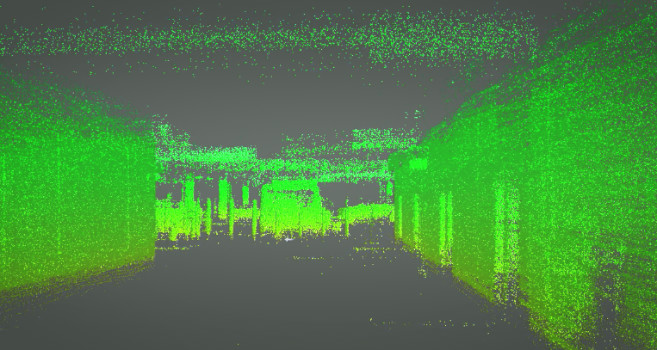
\includegraphics[width=0.6\textwidth]{\pathTech/LIDAR.jpg}
    \caption{Reconstitution d'un intérieur avec un scanner LIDAR.}
\end{figure}
Les principaux avantages de ces techniques sont leurs précisions ainsi que l'adaptabilité à l'environnement. Pour la précision on peut aller jusqu'à 10 cm avec un scanner de type LIDAR.
\medskip
\\
Cependant, les infrarouges admettent des interférences avec la lumière du jour rendant difficile sont utilisation en plein soleil. Son prix est aussi non négligeable, un scanner LIDAR coûte autour de 180 euros la pièce. Pour des capteurs et récepteurs IR plus classiques leurs prix varient entre 3 et 10 euros pièce.